\renewcommand{\theequation}{\theenumi}
\begin{enumerate}[label=\arabic*.,ref=\thesubsection.\theenumi]
\numberwithin{equation}{enumi}
\item Draw a circle with centre $\vec{B}$ and radius 6.  If $\vec{C}$ be  a point 10 units  away from its 
centre, construct the pair of tangents $AC$ and $CD$ to the 
circle.
\\
\solution The tangent is perpendicular to the radius.
%
From the given information, in $\triangle ABC, AC \perp AB, a = 
10$ and $c = 6$.
\begin{align}
b =  \sqrt{a^2-c^2}
\end{align}
The following code plots Fig. \ref{fig:circle}
\begin{lstlisting}
codes/circle/draw_circle_eg.py
\end{lstlisting}
\begin{figure}[!ht]
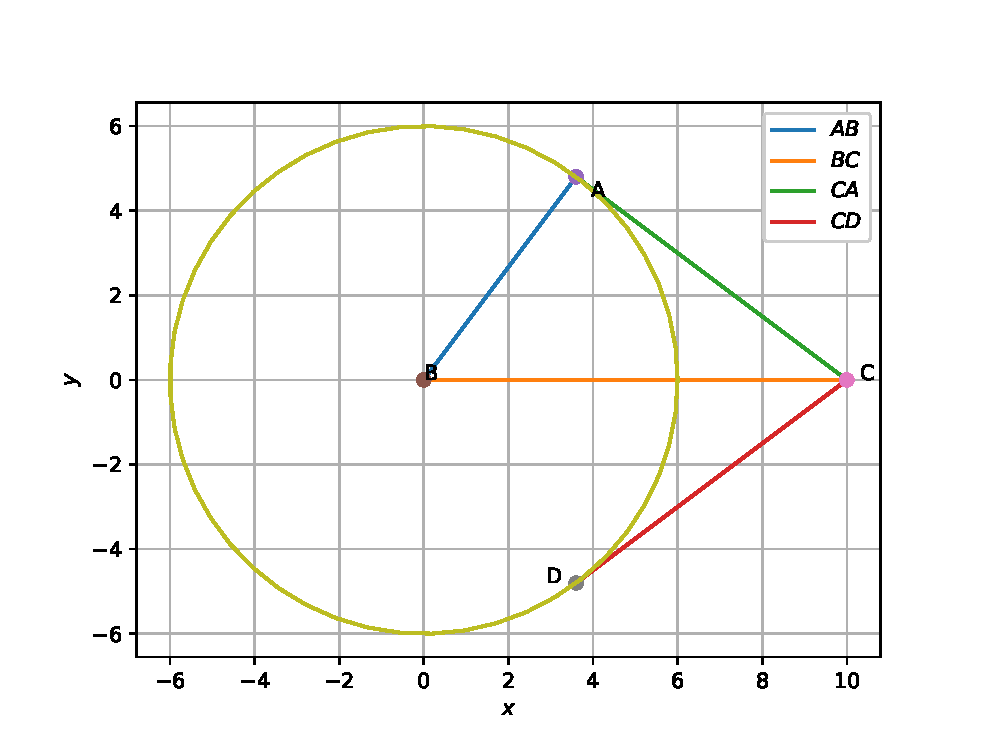
\includegraphics[width=\columnwidth]{./circle/figs/circle.eps}
\caption{}
\label{fig:circle}
\end{figure}
\item Draw a circle of radius 3.  Mark any point $\vec{A}$ on the circle, point  $\vec{B}$ inside the circle  and point  $\vec{C}$ outside the circle.
\\
\solution 
For any angle $\theta$, a point on the circle with radius 3 has coordinates
\begin{align}
3\myvec{\cos \theta\\ \sin\theta}
\end{align}
